\subsection{Salida}
    \begin{figure}[ht]
        \begin{adjustbox}{addcode={
            \begin{minipage}{\width}}{
                \caption{Salida de los tiempos en serie y paralelo con el error}
            \end{minipage}},rotate=360,center}
            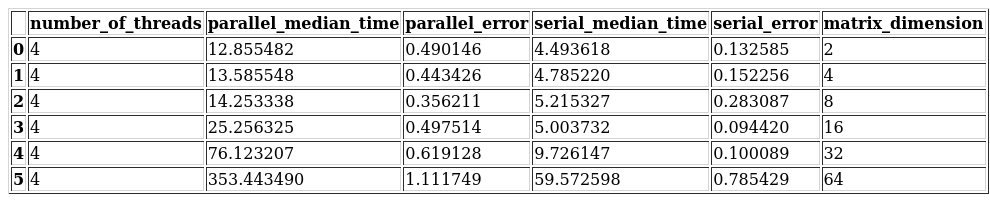
\includegraphics[scale=.6]{gustafson_output_table.png}
        \end{adjustbox}
    \end{figure}
    \FloatBarrier

    Podemos observar que la sección serie del problema se mantiene constante
    mientras que la sección paralela varía en forma lineal con la dimension de
    las matrices de entrada.

    \begin{figure}[ht]
        \begin{adjustbox}{addcode={
            \begin{minipage}{\width}}{
                \caption{Tiempos en serie y paralelo}
            \end{minipage}},rotate=360,center}
            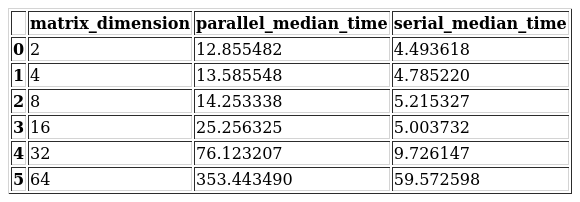
\includegraphics[scale=.6]{gustafson_exec_time_table.png}
        \end{adjustbox}
    \end{figure}
    \FloatBarrier
    \begin{figure}[ht]
        \begin{adjustbox}{addcode={
            \begin{minipage}{\width}}{
                \caption{Tiempo paralelo y serie en funcion de la dimension de las matrices de entrada}
            \end{minipage}},rotate=360,center}
            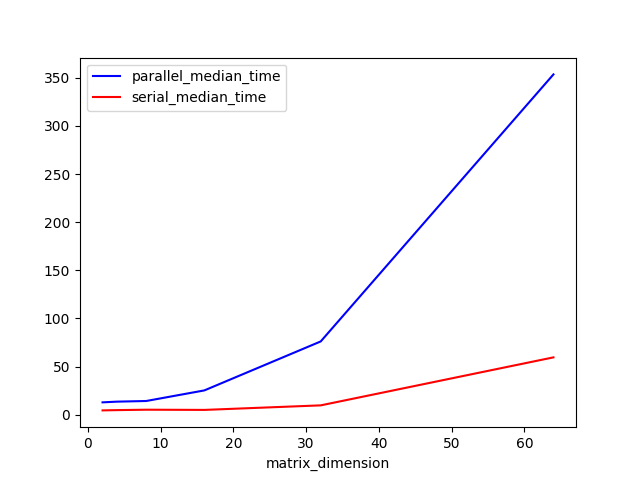
\includegraphics[scale=.6]{gustafson_exec_time.png}
        \end{adjustbox}
    \end{figure}
    \FloatBarrier

    Luego a partir de estos datos podemos calcular el speed up y obtuvimos lo
    siguiente:

    \begin{figure}[ht]
        \begin{adjustbox}{addcode={
            \begin{minipage}{\width}}{
                \caption{Tabla de valores del speed up}
            \end{minipage}},rotate=360,center}
            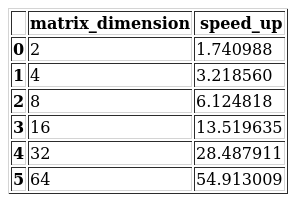
\includegraphics[scale=.6]{gustafson_speed_up_table.png}
        \end{adjustbox}
    \end{figure}
    \FloatBarrier
    \begin{figure}[ht]
        \begin{adjustbox}{addcode={
            \begin{minipage}{\width}}{
                \caption{Grafico del speed up}
            \end{minipage}},rotate=360,center}
            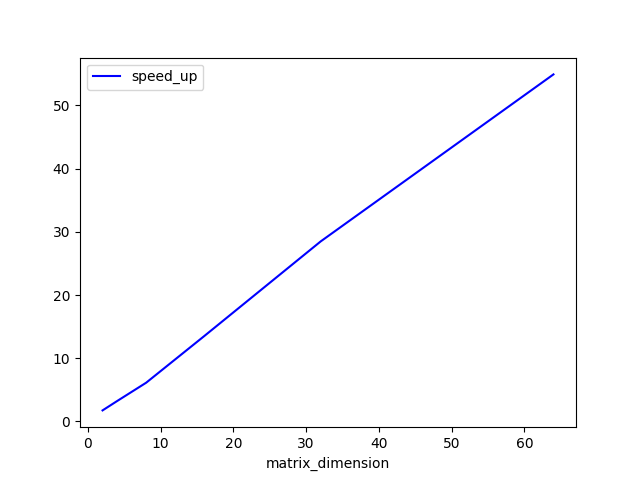
\includegraphics[scale=.6]{gustafson_speed_up.png}
        \end{adjustbox}
    \end{figure}
    \FloatBarrier
